%Copyright (c) 2006 Rice University
%All Rights Reserved
%This code is covered by the Rice-WARP license
%See http://warp.rice.edu/license/ for details
\section{Setting up the Project in XPS}
	\subsection{Create New Project}
		\begin{enumerate}
			%Step 1
			\item Start XPS via \textbf{Program Files} $\rightarrow$ \textbf{Xilinx Platform Studio 8.1i} $\rightarrow$ \textbf{Xilinx Platform Studio}
			%Step 2
			\item At the \textbf{Create new or open existing project} window, select \textbf{Base System Builder} wizard (recommended) and click \textbf{OK}


			
\begin{figure}[htp]
	\centering
	
		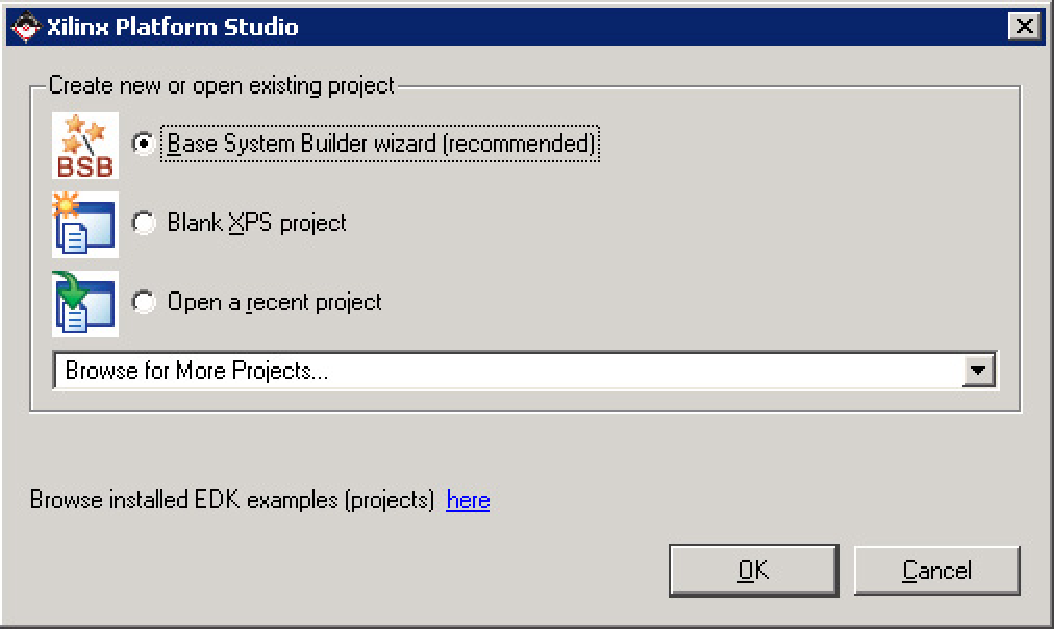
\includegraphics[width=1.00\textwidth]{SWScreenshots/SW1p2.pdf}
	\caption{Step 2 -- Opening Dialog Box}	
	\label{fig:SW1p2}
\end{figure}

			%Step 3
			\item For \textbf{Project file}, Either:
				\begin{enumerate}
					\item Enter: \textbf{C:/WARP/BoardTests/IOTest/system.xmp}.  \\Click \textbf{OK} and click \textbf{Yes} when asked if you would like to create the directory; OR
					\item Browse to the directory in which you would like to store your project. Create a new folder within this directory and open it. The file name should be system.xmp. Click \textbf{Save}. XPS will save all the various project files and folders in this project folder. Click \textbf{OK} to move to tthe next window.
					\item This readme assumes method one when giving locations.  You must adjust your addresses accordingly if choosing to save the system elsewhere.
				\end{enumerate}
			
\begin{figure}[htp]
	\centering
		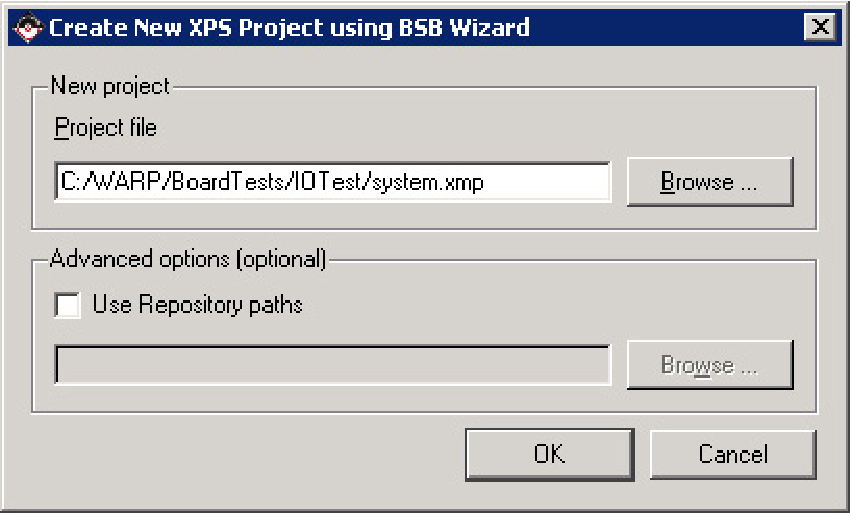
\includegraphics[width=.75\textwidth]{SWScreenshots/SW1p3a.pdf}
	\caption{Step 3 -- Choose a directory for \textit{system.xmp}}
	\label{fig:SW1p3a}
\end{figure}

\begin{figure}[htp]
	\centering
		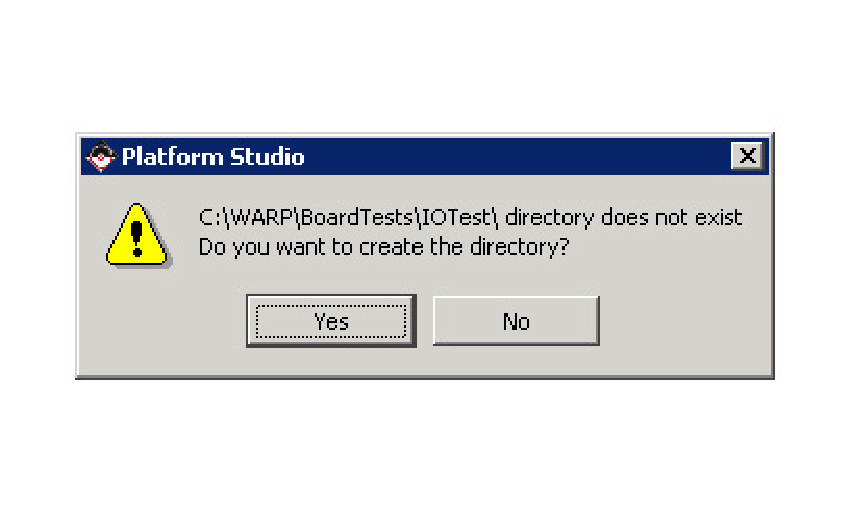
\includegraphics[width=.75\textwidth]{SWScreenshots/SW1p3b.pdf}
	\caption{Step 3 -- Click \textbf{Yes} to create the directory.}
	\label{fig:SW1p3b}
\end{figure}

			\newpage
			%Step4%%%%%%%%%%%%%%%%%%%%%%%%%%%%%%%%%%%%%%				
			\item The \textbf{Base System Builder - Welcome} window should appear. Select \textbf{I would like to create a new design}, and click \textbf{Next}
\vspace{.5in}			
\begin{figure}[htbp]
	\centering
		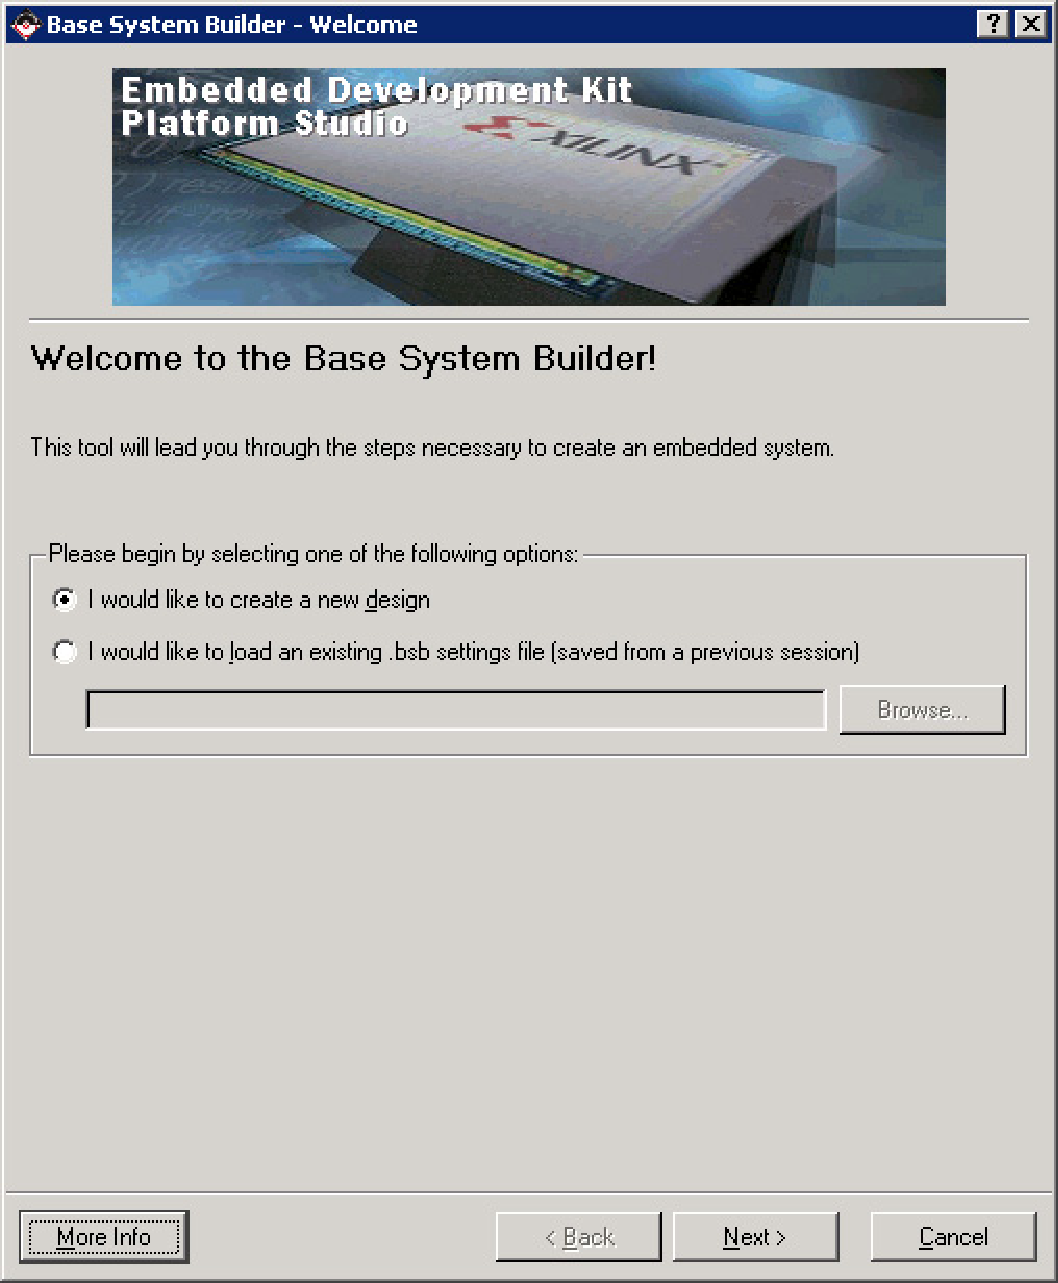
\includegraphics[width=.80\textwidth]{SWScreenshots/SW1p4.pdf}
	\caption{Step 4 -- Welcome Screen}
	\label{fig:SW1p4}
\end{figure}
			
			\newpage
			%Step 5%%%%%%%%%%%%%%%%%%%%%%%%%%%%%%%%%%%%%%%%
			\item At the \textbf{Select Board} window, make the following selections and click \textbf{Next}:
				\begin{itemize}
					\item Board vendor: \textit{Rice University CMC - WARP Project}
					\item Board name: \textit{WARP FPGA and Radio Boards}
					\item Board revision: \textit{1.0b}
				\end{itemize}
				\vspace{.25in}
\begin{figure}[htbp]
	\centering
		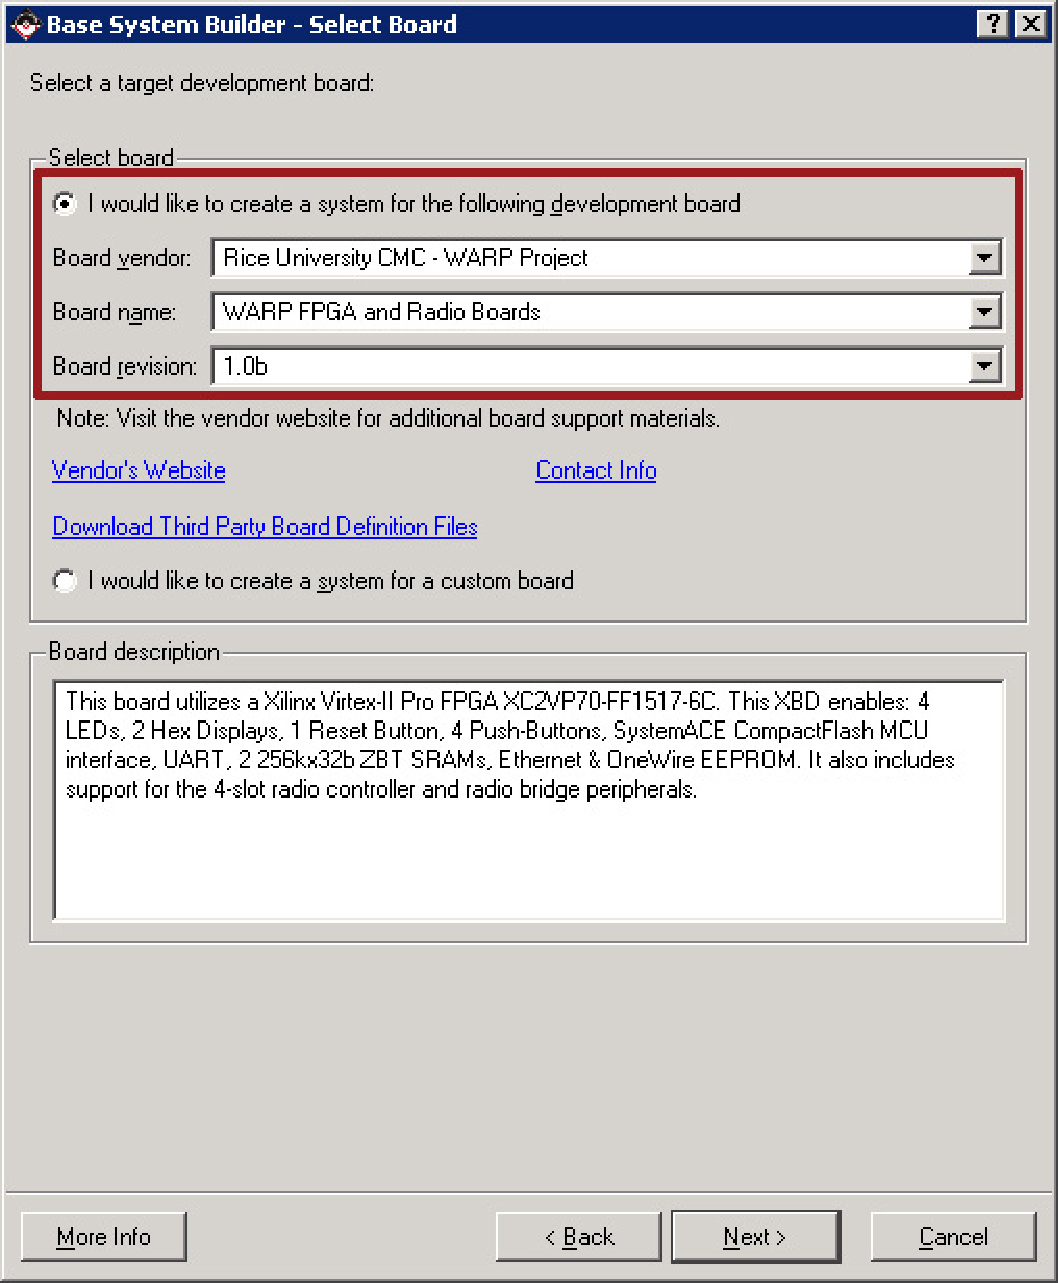
\includegraphics[width=.8\textwidth]{SWScreenshots/SW1p5.pdf}
\caption{Step 5 -- \textbf{Select Board} window}
\label{fig:SW1p5}
\end{figure}
			
			\newpage
			%Step 6	
			\item Make sure \textbf{PowerPC} is your selected processor. Click \textbf{Next}
			\vspace{.5in}
\begin{figure}[htbp]
	\centering
		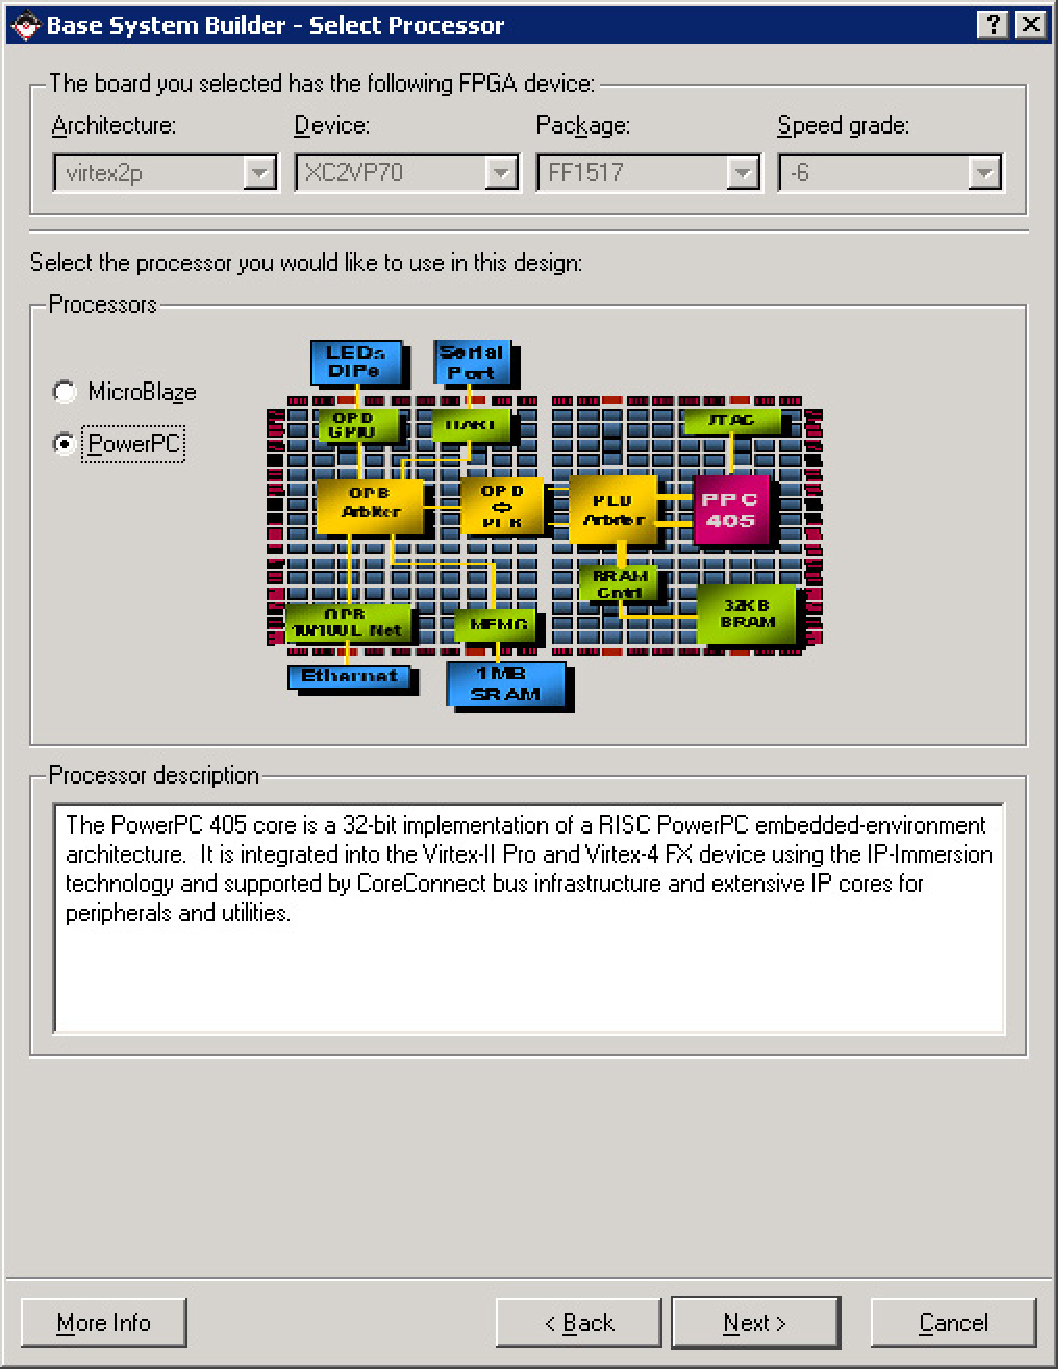
\includegraphics[width=.8\textwidth]{SWScreenshots/SW1p6.pdf}
	\caption{Step 6 -- Processor Selection window}
	\label{fig:SW1p6}
\end{figure}
			
			\newpage
			%Step 7
			\item The \textbf{Configure PowerPC} window should appear, make the following designations and click \textbf{Next}:
				\begin{itemize}
					\item Processor clock frequency: \textit{100.00 MHz}
					\item Bus clock frequency: \textit{50.00 MHz}
					\item Processor configuration: \textit{FPGA JTAG}
					\item On-chip memory (OCM)
						\begin{itemize}
							\item Data: \textit{64 KB}
							\item Instruction: \textit{128 KB}
						\end{itemize}
					\item Cache setup should be \textit{unchecked}
				\end{itemize}
			
			
\begin{figure}[htbp]
	\centering
		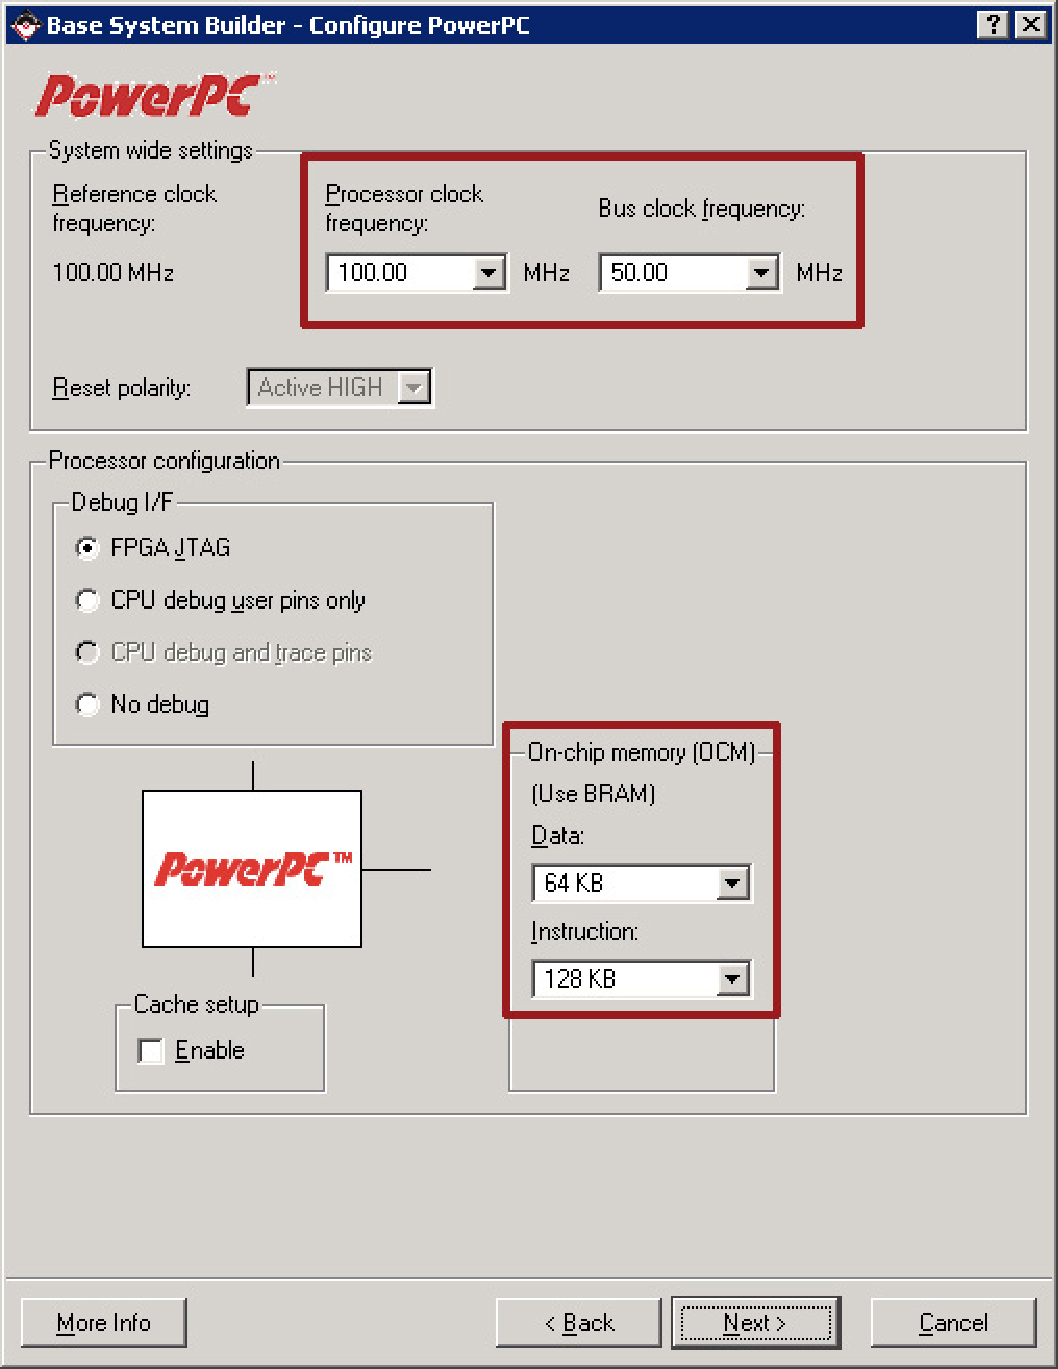
\includegraphics[width=.70\textwidth]{SWScreenshots/SW1p7.pdf}
	\caption{Step 7 -- Configure PowerPC}
	\label{fig:SW1p7}
\end{figure}

			\newpage
			%Step 8	
			\item The next windows are \textbf{Configure IO Interfaces}. Depending on the size of your window, a varying number of IO devices will be available on each screen. Make sure the following are checked (if an attribute is not enumerated, assume default configuration):
				\begin{itemize}
					\item \textit{LED\_7SEGMENT}
					\item \textit{LED\_7SEGMENT\_1}
					\item \textit{LEDs\_4Bit}
					\item \textit{Push\_Buttons\_4bit}
						\begin{itemize}
							\item Check \textbf{Use interrupt} for the Push\_buttons\_4bit IO device.\\ IMPORTANT: If you fail to do so now, consult the Help Documentation to learn how to add them once the project is created.
						\end{itemize}
					\item \textit{RS232}
						\begin{itemize}
							\item Peripheral: \textit{OPB UARTLITE}
							\item Baudrate: \textit{57600}
						\end{itemize}
					\item \textit{DIPSWs\_4bit}
					\item \textbf{UNCHECK}: \textit{SysACECompactFlash}, \textit{Ethernet\_MAC},\textit{onewire\_0}, \\\textit{radio\_controller\_0}, \textit{radio\_bridge\_slot\_2}, \textit{SRAM0\_ZBT\_512Kx32}, \\and \textit{SRAM1\_ZBT\_512Kx32} 
				\end{itemize}
	
\begin{figure}[htbp]
	\centering
		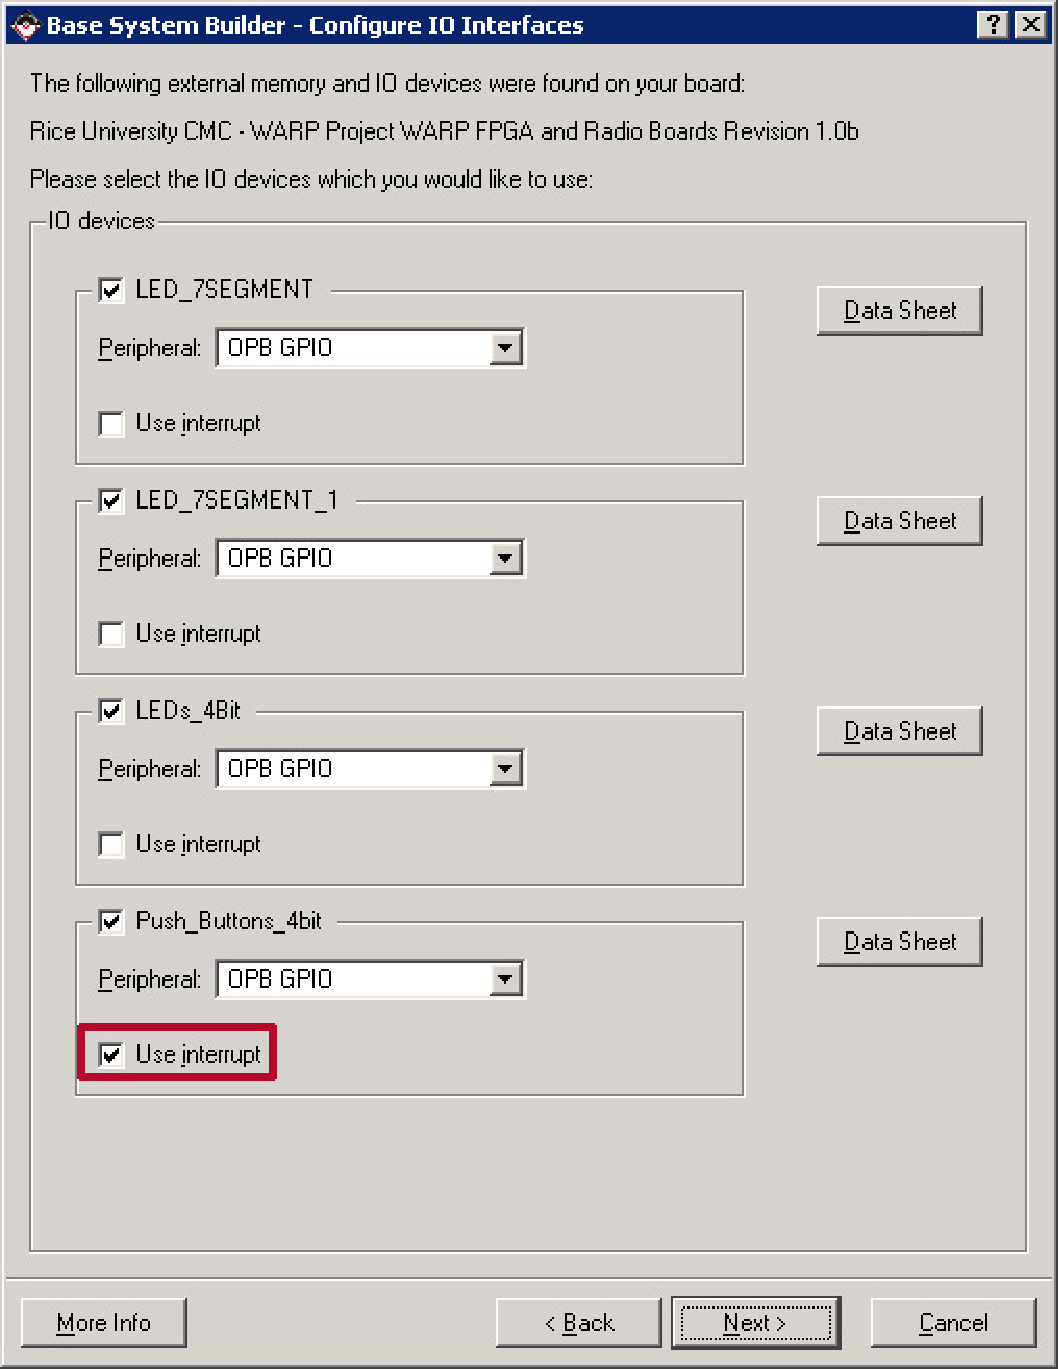
\includegraphics[width=.9\textwidth]{SWScreenshots/SW1p8a.pdf}
	\caption{Step 8 -- Choosing Peripherals}
	\label{fig:SW1p8a}
\end{figure}

\begin{figure}[htbp]
	\centering
		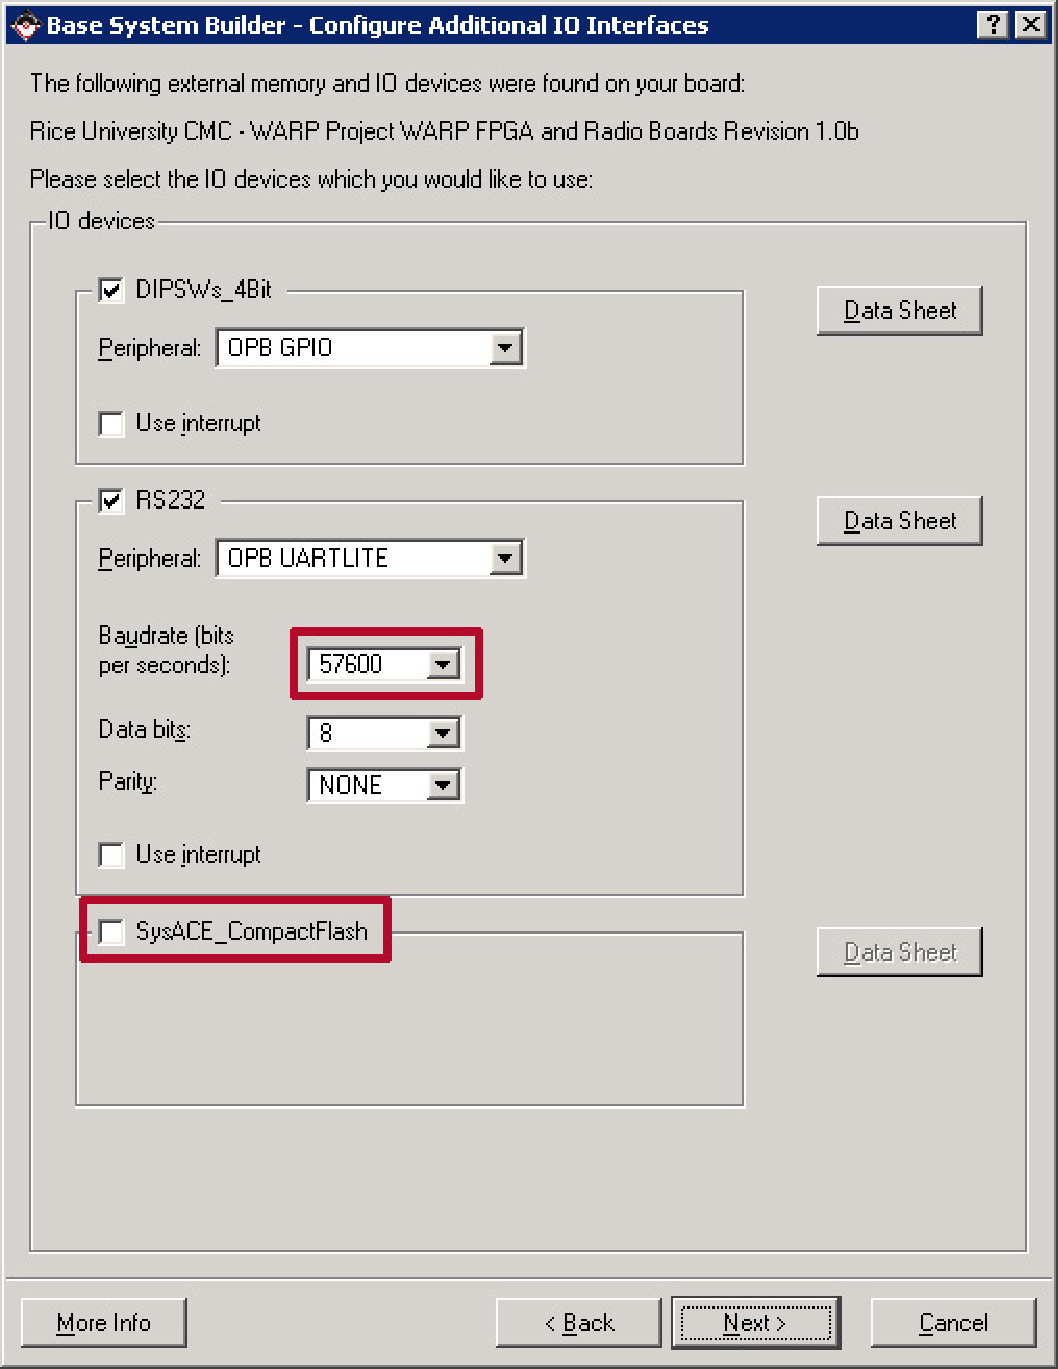
\includegraphics[width=.9\textwidth]{SWScreenshots/SW1p8b.pdf}
	\caption{Step 8 -- Choosing Peripherals cont.}
	\label{fig:SW1p8b}
\end{figure}

\begin{figure}[htbp]
	\centering
		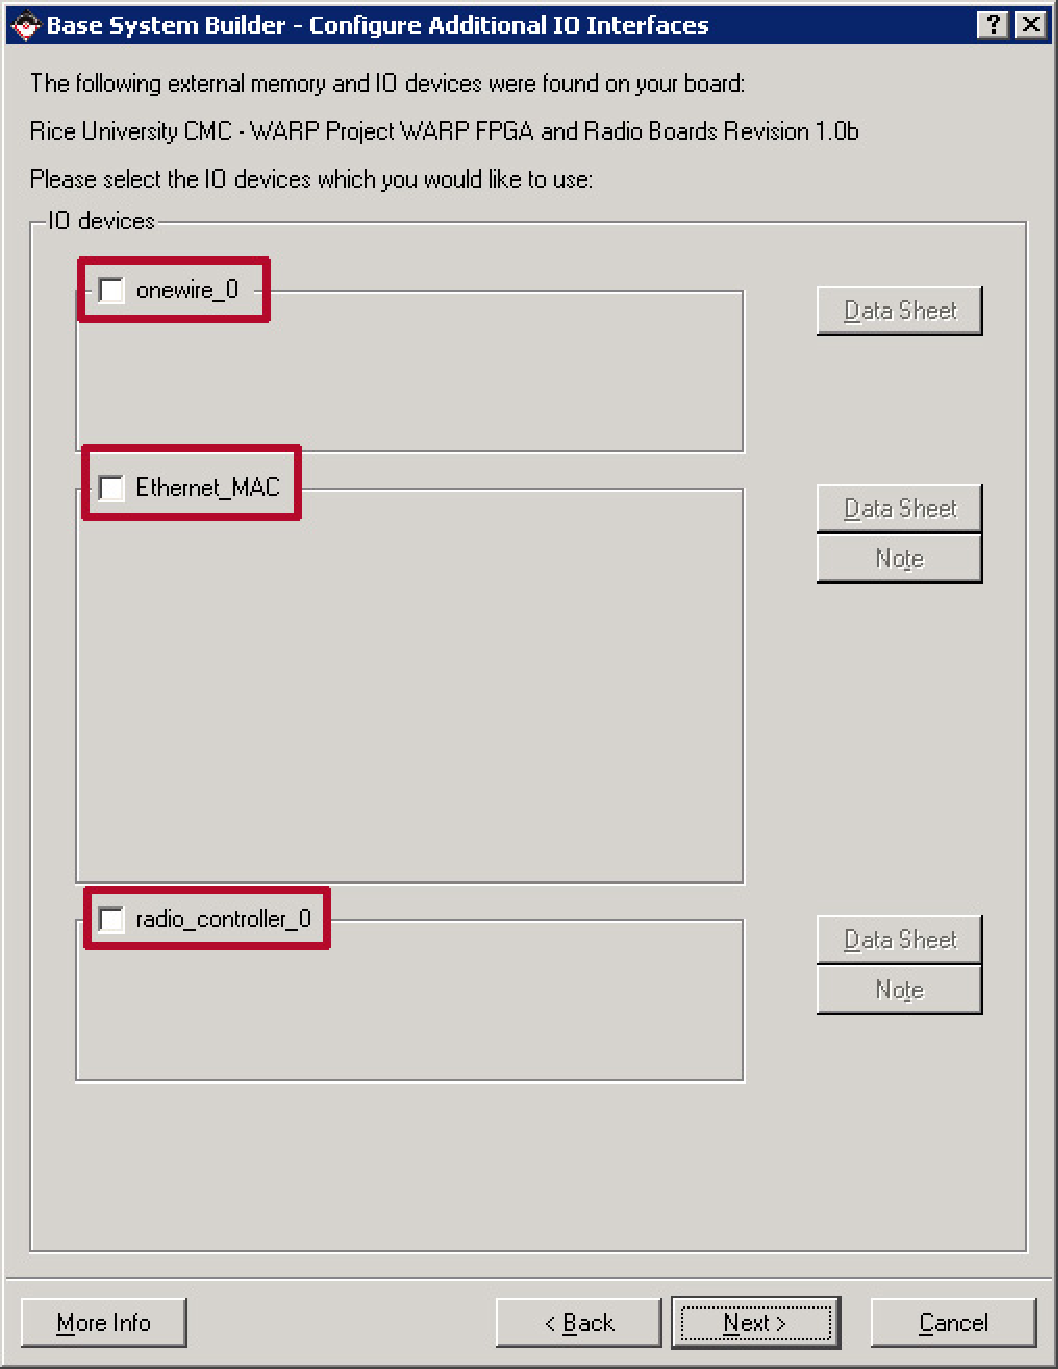
\includegraphics[width=.9\textwidth]{SWScreenshots/SW1p8c.pdf}
	\caption{Step 8 -- Choosing Peripherals cont.}
	\label{fig:SW1p8c}
\end{figure}

\begin{figure}[htbp]
	\centering
		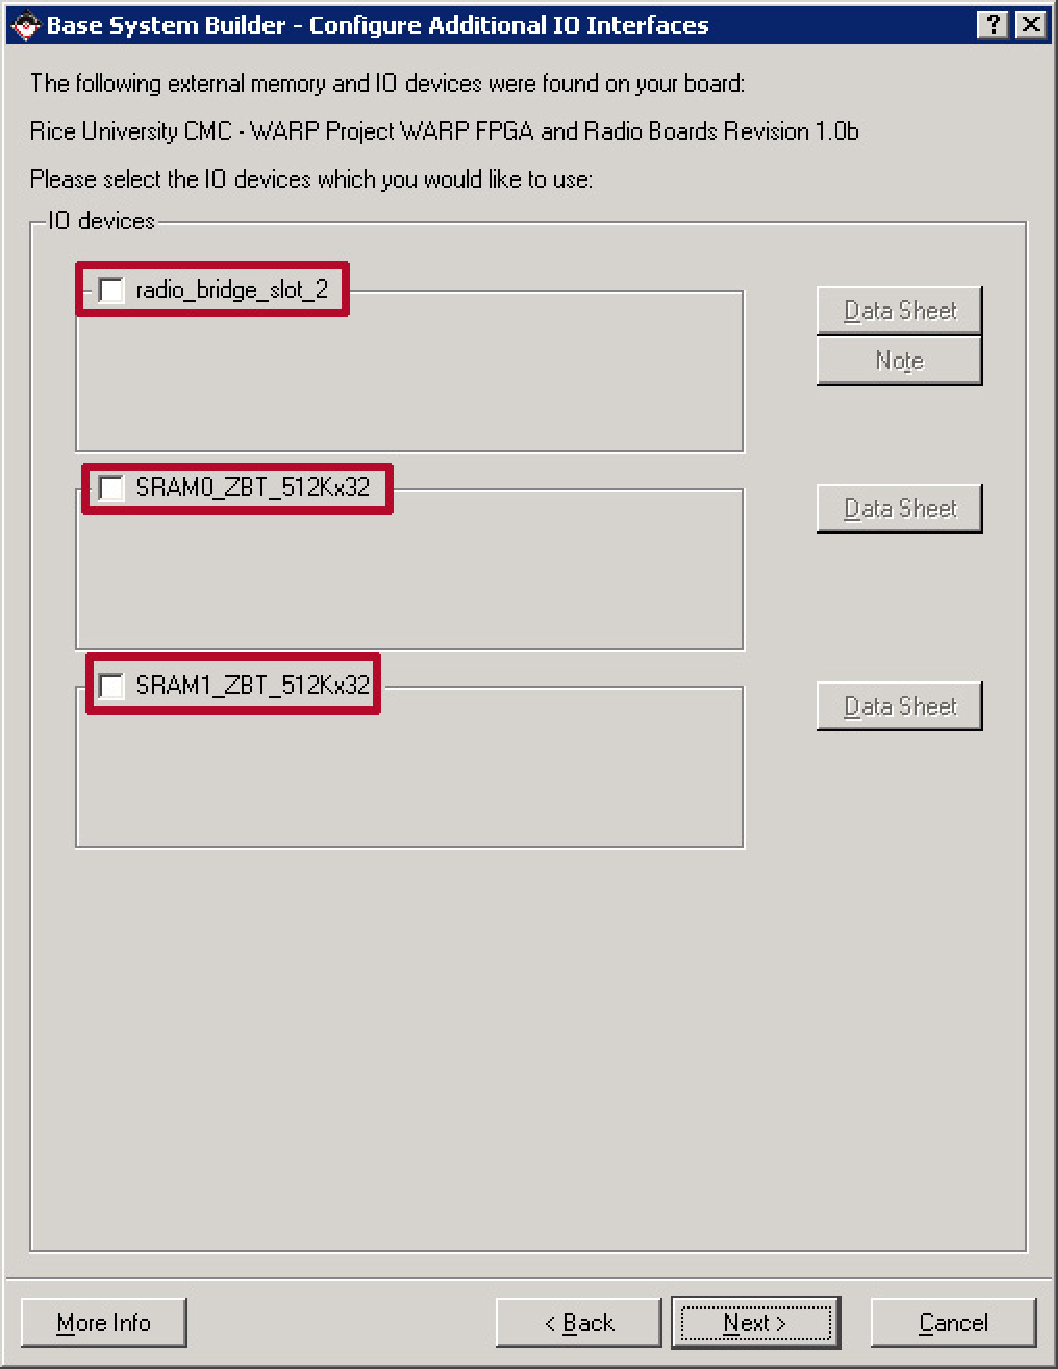
\includegraphics[width=.9\textwidth]{SWScreenshots/SW1p8d.pdf}
	\caption{Step 8 -- Choosing Peripherals cont.}
	\label{fig:SW1p8d}
\end{figure}

			\newpage
			%Step 9
			\item At \textbf{Add Internal Peripherals}, click \textbf{Remove} to the right of the\\ \textbf{plb\_bram\_if\_cntlr\_1 box}. Click \textbf{Next}
\vspace{.25in}
\begin{figure}[htbp]
	\centering
		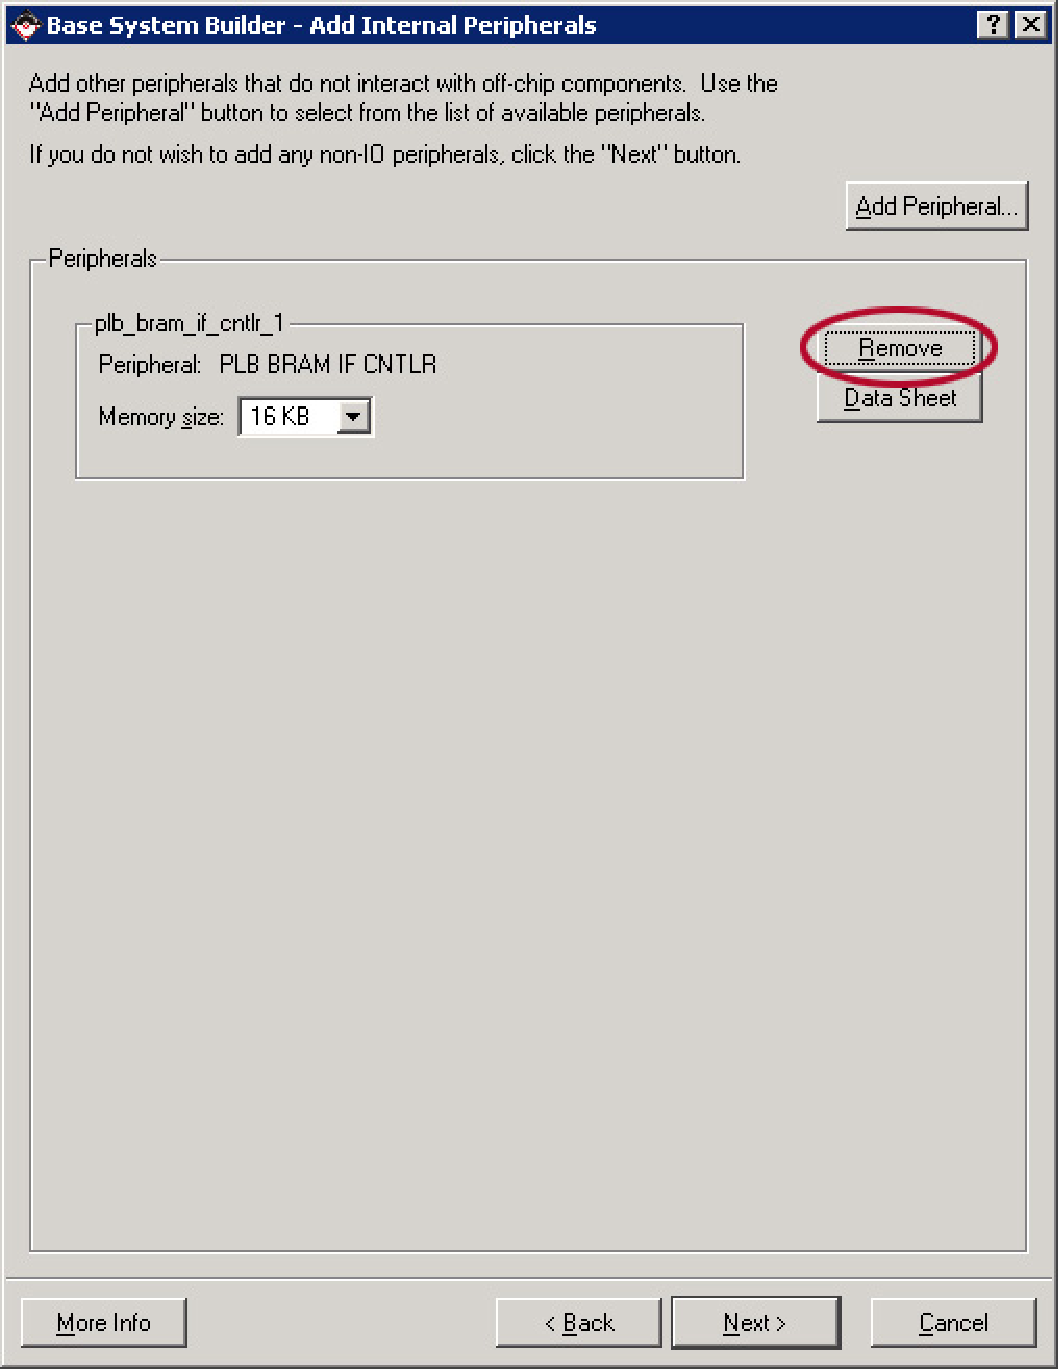
\includegraphics[width=.80\textwidth]{SWScreenshots/SW1p9a.pdf}
	\caption{Step 9 -- Before Removing}
	\label{fig:SW1p9a}
\end{figure}

\begin{figure}[htbp]
	\centering
		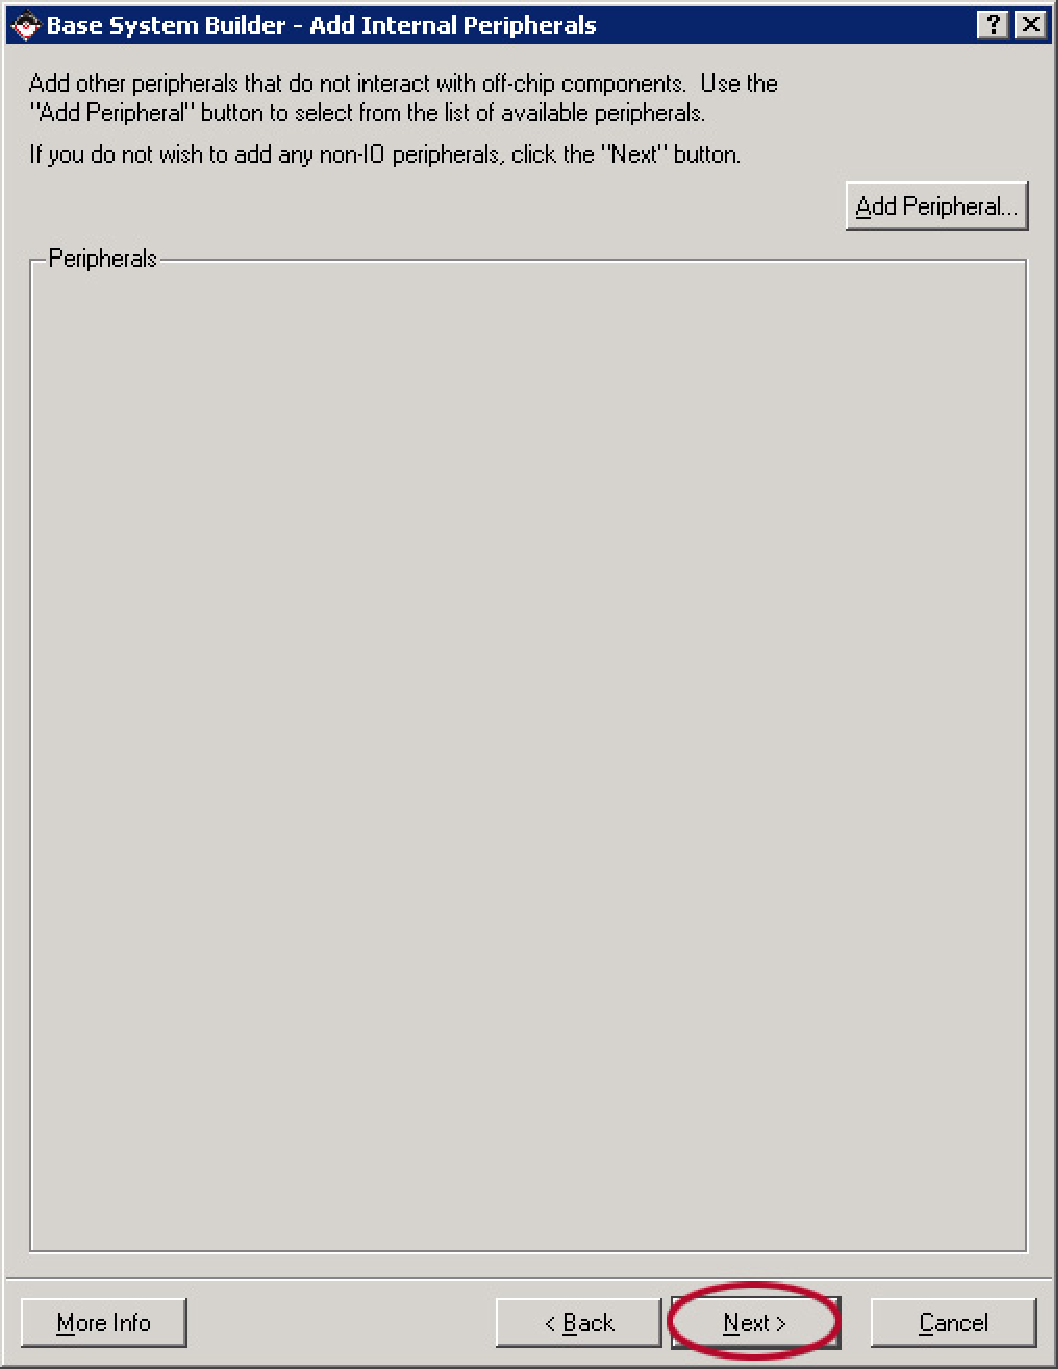
\includegraphics[width=.80\textwidth]{SWScreenshots/SW1p9b.pdf}
	\caption{Step 9 -- After Removing}
	\label{fig:SW1p9b}
\end{figure}
			
			
			\newpage
			%Step 10%%%%%%%%%%%%%%%%%%%%%%%%%%%%%%%%
			\item At \textbf{Software Setup}, UNCHECK \textbf{Memory test} and \textbf{Peripheral selftest}. \textbf{RS232} should be chosen for \textbf{STDIN} and \textbf{STDOUT}. Click \textbf{Next}.
\vspace{.25in}
\begin{figure}[htbp]
	\centering
		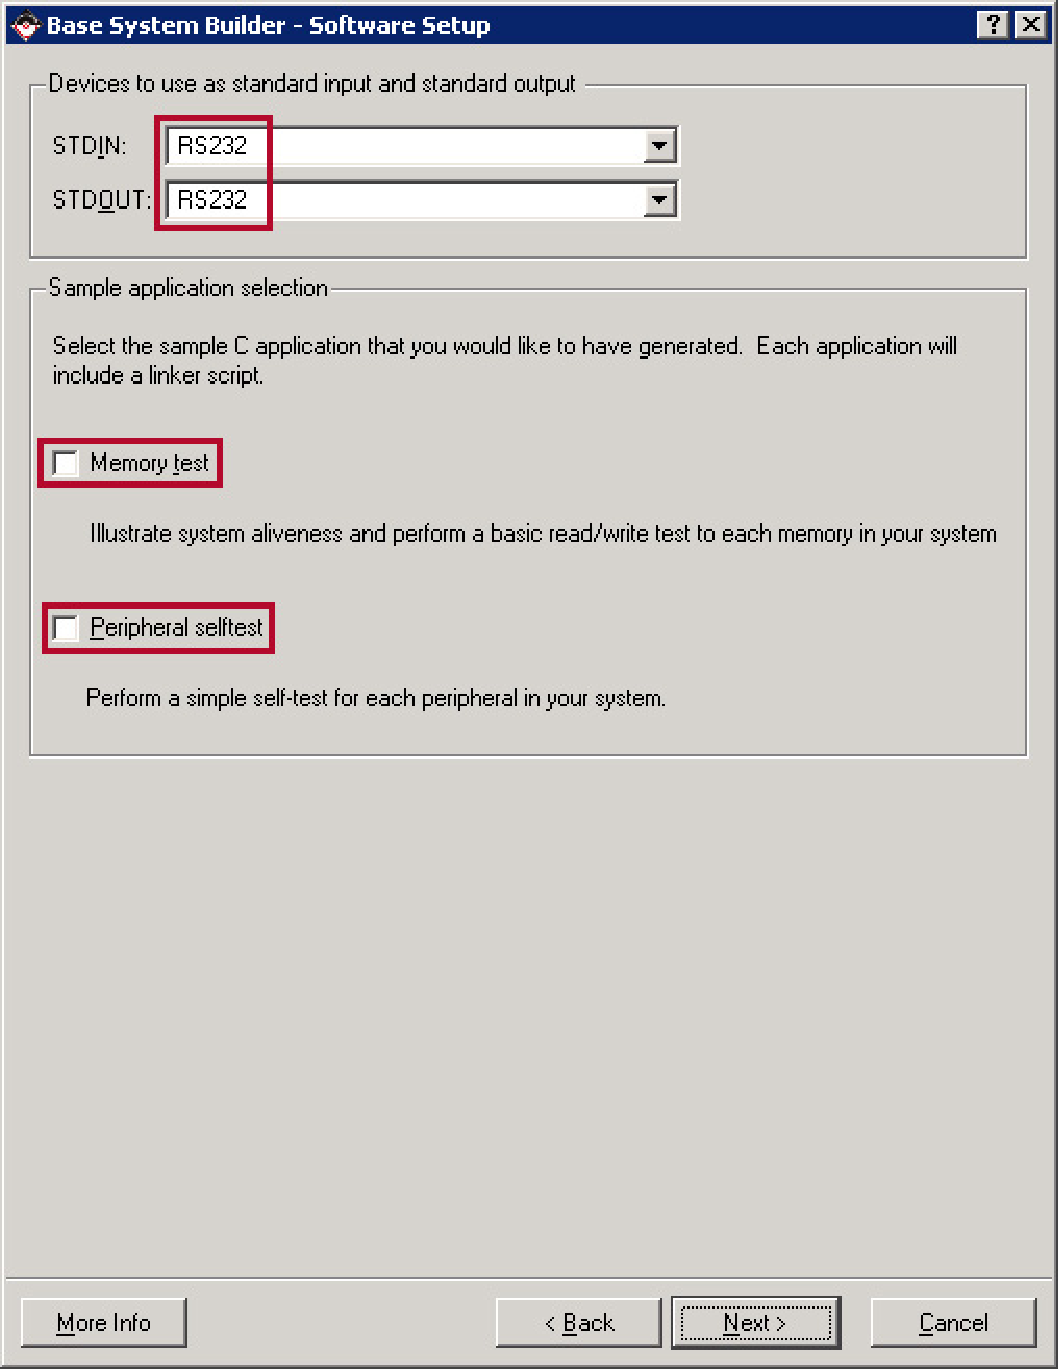
\includegraphics[width=.80\textwidth]{SWScreenshots/SW1p10.pdf}
	\caption{Step 10 -- Software Setup}
	\label{fig:SW1p10}
\end{figure}
			
			\newpage
			%Step 11
			\item If you chose to keep the ``Memory test'' or ``Peripheral selftest'' simply click \textbf{NEXT} through configuration menu(s). Click \textbf{Generate} at the \textbf{System Created} window. Click \textbf{Finish} to exit the builder. Click \textbf{OK} to beging using XPS.
		\end{enumerate}

\begin{figure}[htbp]
	\centering
		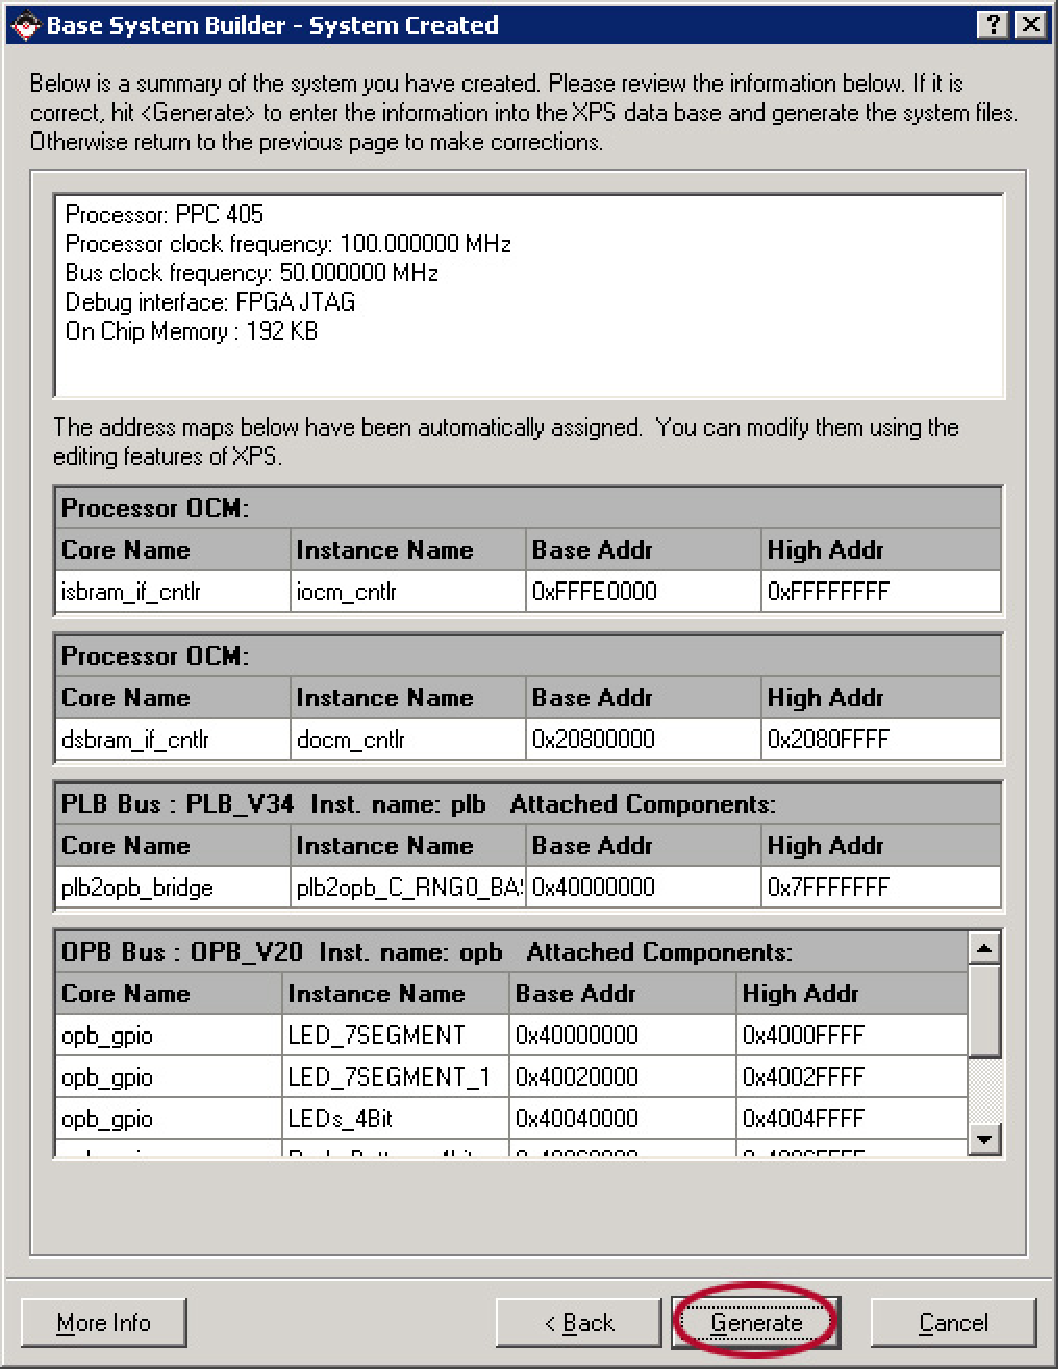
\includegraphics[width=.80\textwidth]{SWScreenshots/SW1p11a.pdf}
	\caption{Step 11 -- Generate File}
	\label{fig:SW1p11a}
\end{figure}

\begin{figure}[htbp]
	\centering
		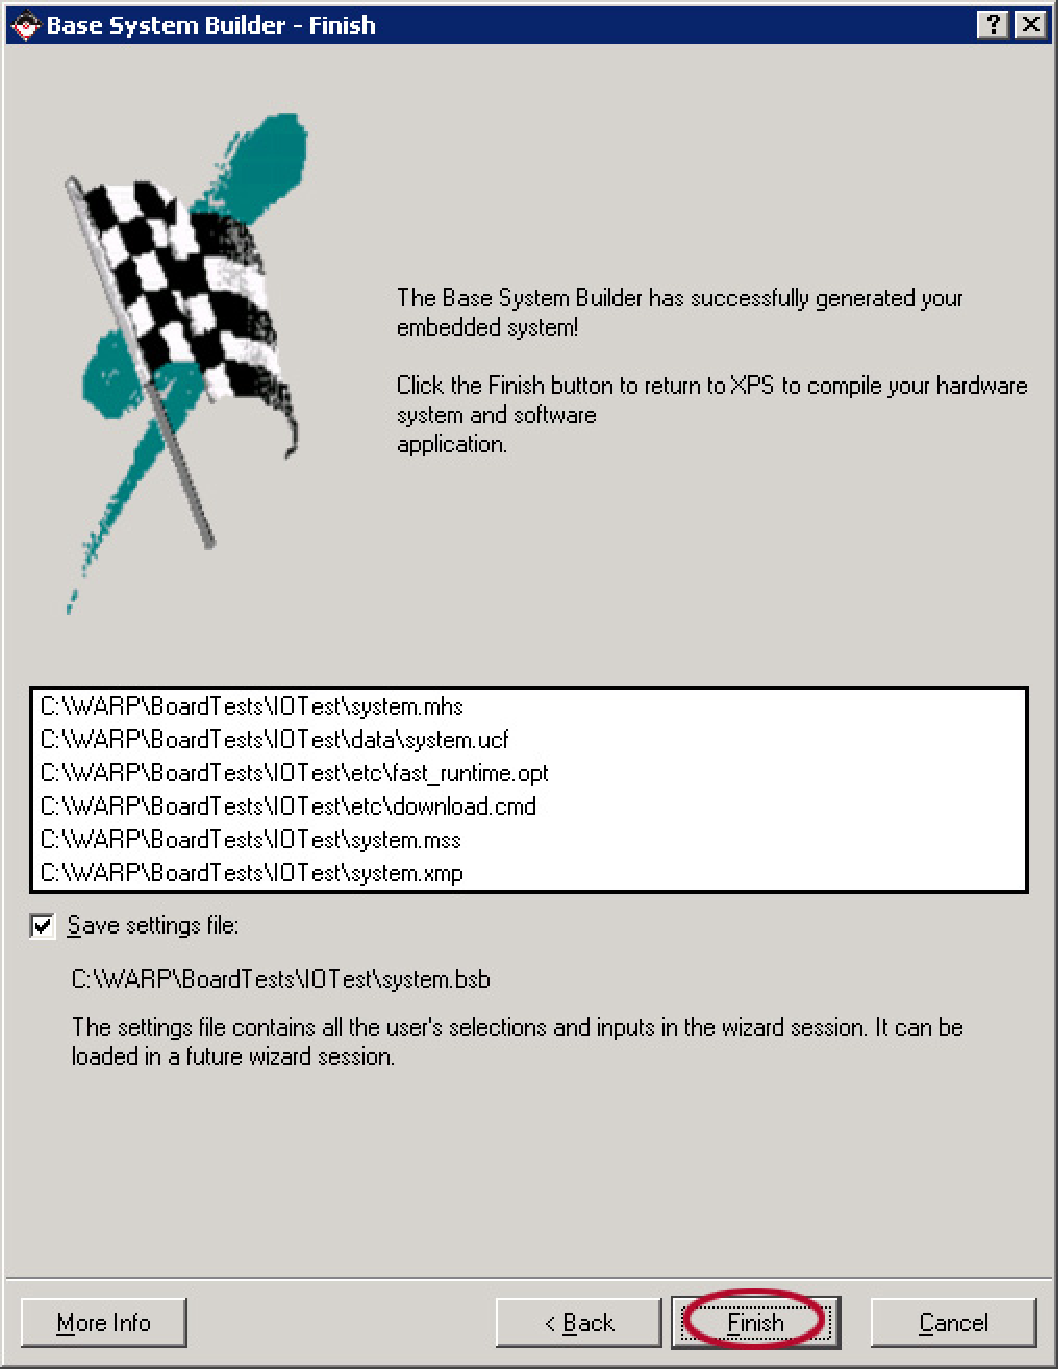
\includegraphics[width=.80\textwidth]{SWScreenshots/SW1p11b.pdf}
	\caption{Step 11 -- Finish}
	\label{fig:SW1p11b}
\end{figure}

\begin{figure}[htbp]
	\centering
		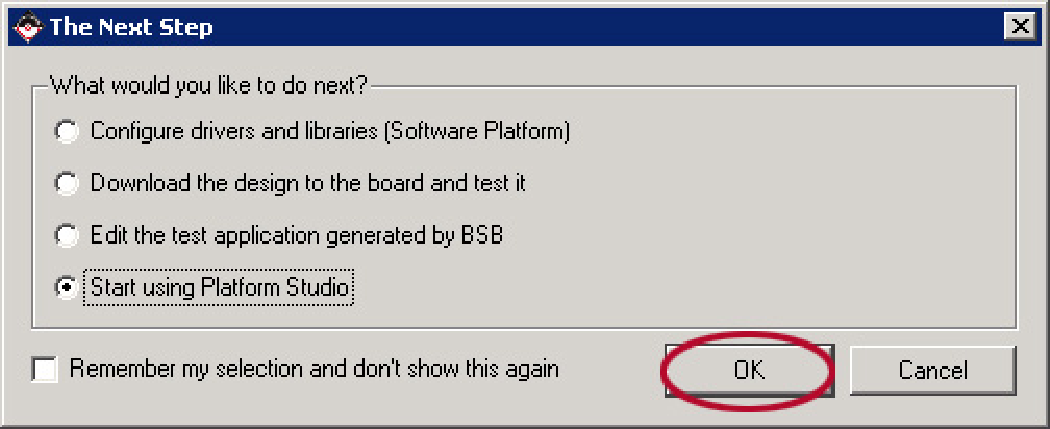
\includegraphics[width=1.00\textwidth]{SWScreenshots/SW1p11c.pdf}
	\caption{Step 11 -- Start Working}
	\label{fig:SW1p11c}
\end{figure}

\begin{figure}[htbp]
	\centering
		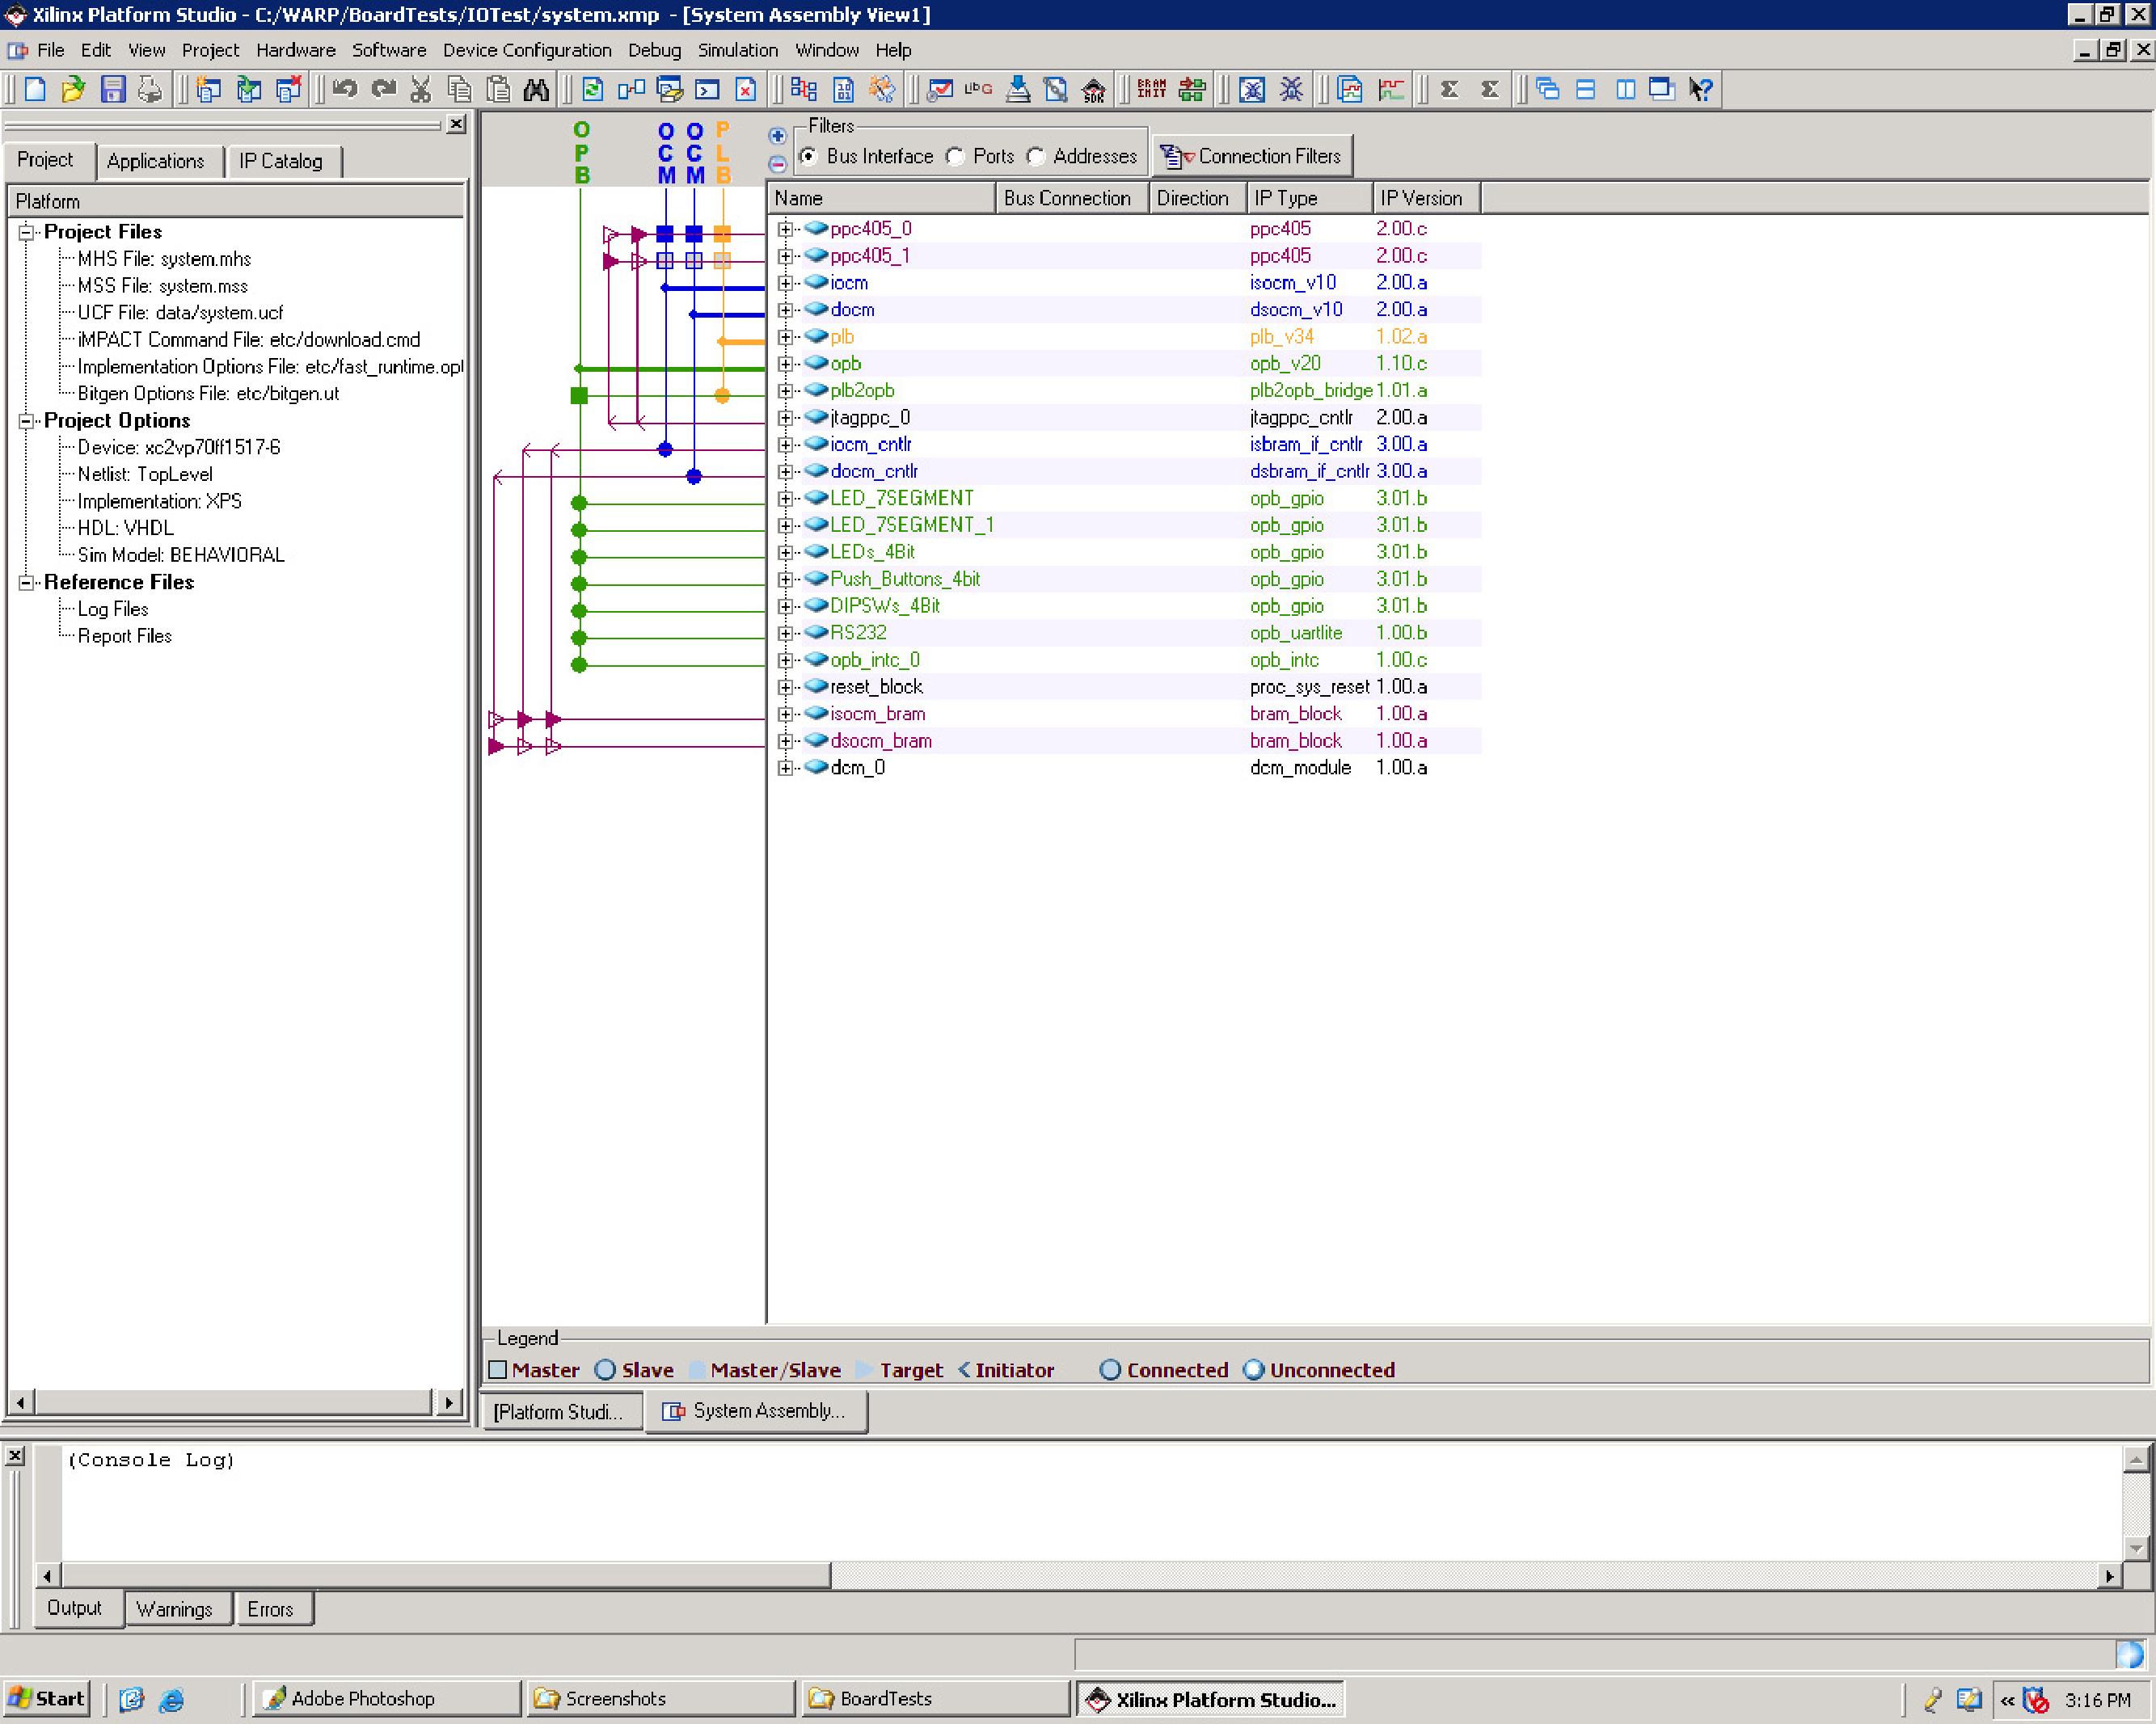
\includegraphics[width=1.00\textwidth]{SWScreenshots/SW1p12.pdf}
	\caption{XPS Workspace after Base System Builder}
	\label{fig:SW1p12}
\end{figure}

	
%%%%%%%%%%%%%%%%%%%%%%%%%%%%%%%%%%%%%%%%%%%%%%%%%%%%%%%%%%%%%%%%%%%%%%%%%%%%%%%%
%New Subsection	
	
	\newpage	
	\subsection{Setting up the UserIO Test in XPS}
		\begin{enumerate}
			
			%Step 1%%%%%%%%%%%%%%%%%%%%%%%%%%%	
			\item Click on the \textbf{Applications} tab in the left hand box. Right-click on \textbf{Add Software Application Project...} and choose \textbf{Add Software Application Project...} Type in \textbf{UserIOTest}, and click \textbf{OK}. You should see you project in the list of ``Software Projects''.
			
\begin{figure}[htbp]
	\centering
		\includegraphics[width=.70\textwidth]{SWScreenshots/SW2p1a.pdf}
	\caption{Step 1 -- Adding a Software Project}
	\label{fig:SW2p1}
\end{figure}

\begin{figure}[htbp]
	\centering
		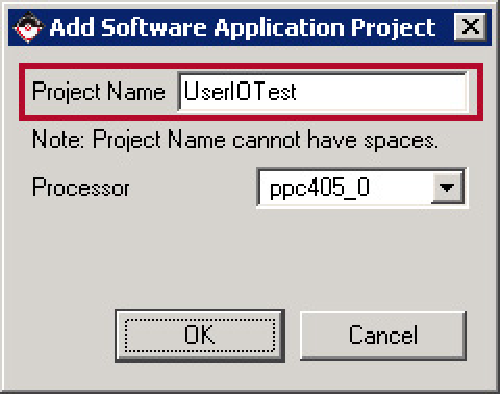
\includegraphics[width=.40\textwidth]{SWScreenshots/SW2p1.pdf}
	\caption{Step 1 -- Name the project: UserIOTest}
	\label{fig:SW2p1a}
\end{figure}

			\newpage
			%Step 2%%%%%%%%%%%%%%%%%%%%%%%%%%%	
			\item Right-click on \textbf{Sources} and choose \textbf{Add Existing Files...} \\Browse to \textbf{c:/WARP/BoardTests/Files}. You will want to add the following *.c files:
				\begin{itemize}
					\item \textit{warplib.c}
					\item \textit{UserIOTest.c}
				\end{itemize}

\begin{figure}[htbp]
	\centering

\includegraphics[width=.40\textwidth]{SWScreenshots/SW2p2a.pdf}
	\caption{Step 2 -- Adding Source Files}
	\label{fig:SW2p2a}
\end{figure}

\begin{figure}[htbp]
	\centering
		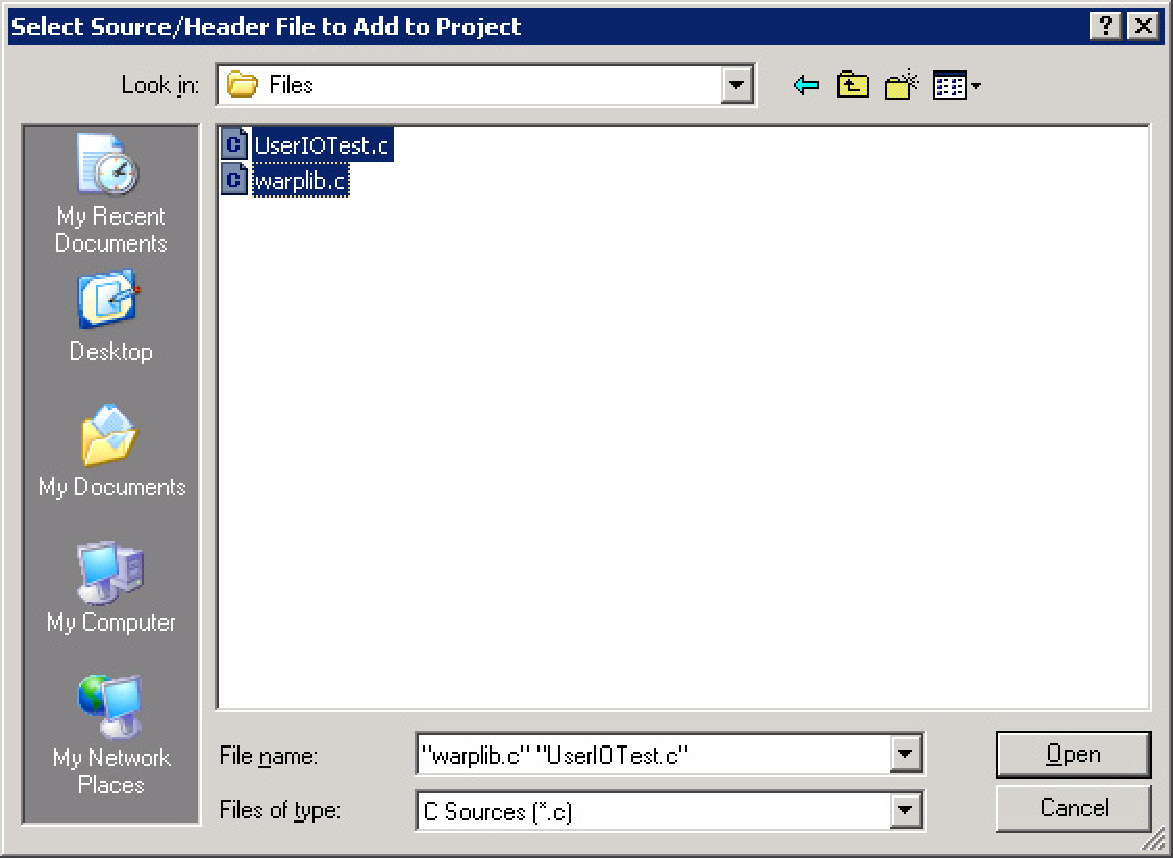
\includegraphics[width=.7\textwidth]{SWScreenshots/SW2p2b.pdf}
	\caption{Step 2 -- Select: UserIOTest.c and warplib.c}
	\label{fig:SW2p2b}
\end{figure}

			\newpage\newpage
			%Step 3%%%%%%%%%%%%%%%%%%%%%%%%%%%	
			\item Next, right-click on \textbf{Headers} and choose \textbf{Add Existing Files...} You should already be in the correct folder.  \\If you do not see \textit{warplib.h}, browse to \textbf{c:/WARP/BoardTests/Files}. You will want to add the following *.h file:
				\begin{itemize}
					\item \textit{warplib.h}
				\end{itemize}
				
				
\begin{figure}[htp]
	\centering
		\includegraphics[width=.40\textwidth]{SWScreenshots/SW2p3a.pdf}
	\caption{Step 3 -- Adding Header Files}
	\label{fig:SW2p3a}
\end{figure}

\begin{figure}[htp]
	\centering
		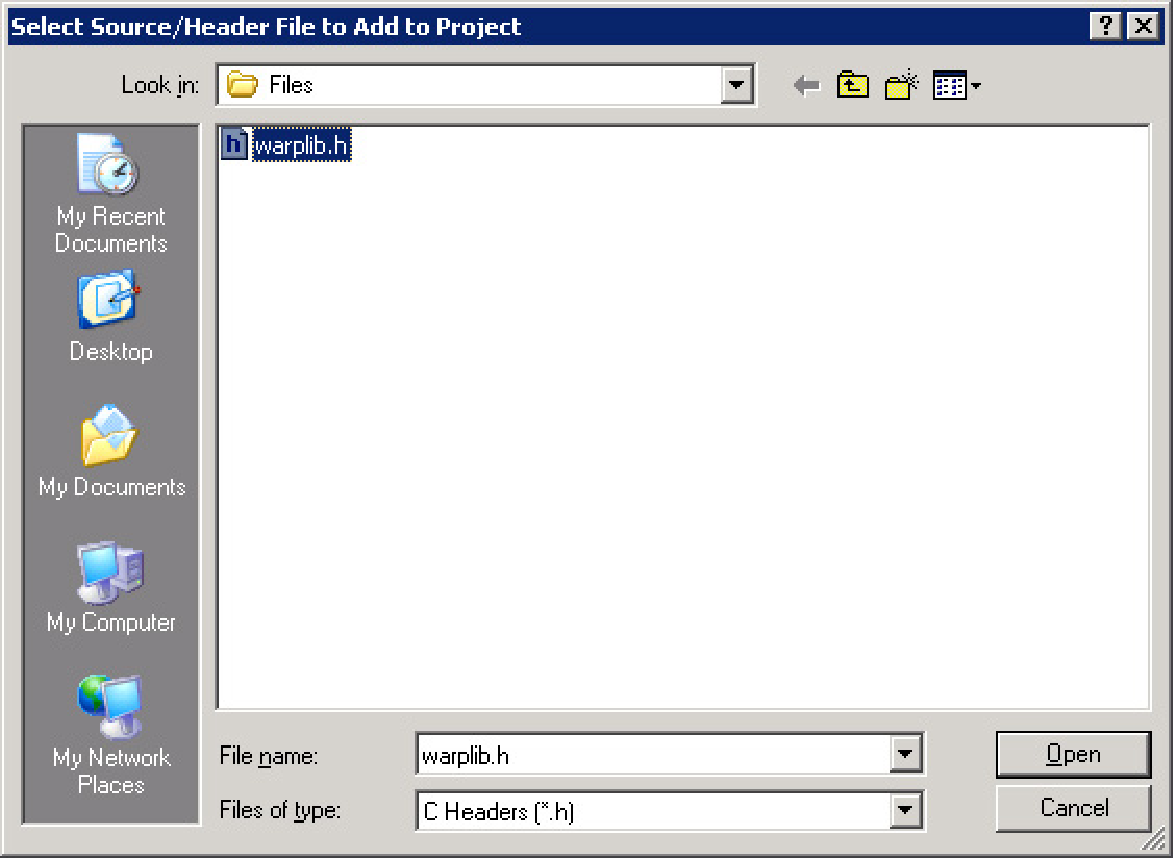
\includegraphics[width=.65\textwidth]{SWScreenshots/SW2p3b.pdf}
	\caption{Step 3 -- Select: warplib.h}
	\label{fig:SW2p3b}
\end{figure}

			\newpage
			%Step 4%%%%%%%%%%%%%%%%%%%%%%%%%%%	
			\item Right-click on \textbf{Default: ppc405\_0\_bootloop} in the right hand menu. Uncheck \textbf{Mark to Intialize BRAMs}.  Afterward, there should be a red `x' over the green arrow next to the name.
			
			
\begin{figure}[htp]
	\centering
		\includegraphics[width=.50\textwidth]{SWScreenshots/SW2p4.pdf}
	\caption{Step 4 -- Uninitializing BRAMs for the Default}
	\label{fig:SW2p4}
\end{figure}

		  %\newpage
			%Step 5%%%%%%%%%%%%%%%%%%%%%%%%%%%	
			\item Right-click on \textbf{Project: UserIOTest} and check \textbf{Mark to Initialize BRAMs}. This step tells XPS to update the bitstream with your project.  Afterward, there should no longer be a red `x' over the green arrow next to the name.
			
			
\begin{figure}[htbp]
	\centering
		\includegraphics[width=.50\textwidth]{SWScreenshots/SW2p5.pdf}
	\caption{Step 5 -- Initializing BRAMs for UserIOTest}
	\label{fig:SW2p5}
\end{figure}

			\newpage
			%Step 6%%%%%%%%%%%%%%%%%%%%%%%%%%%	
			\item Right-click on \textbf{Project: UserIOTest} and select \textbf{Generate Linker Script}. Make sure that each article under the \textbf{Memory} drop down menus is either set to \textbf{iocm\_cntlr} or \textbf{docm\_cntlr}. Click \textbf{Generate}
			
			
\begin{figure}[htp]
	\centering
		\includegraphics[width=.40\textwidth]{SWScreenshots/SW2p6a.pdf}
	\caption{Step 6 -- Generate Linker Script}
	\label{fig:SW2p6a}
\end{figure}

\begin{figure}[htp]
	\centering
		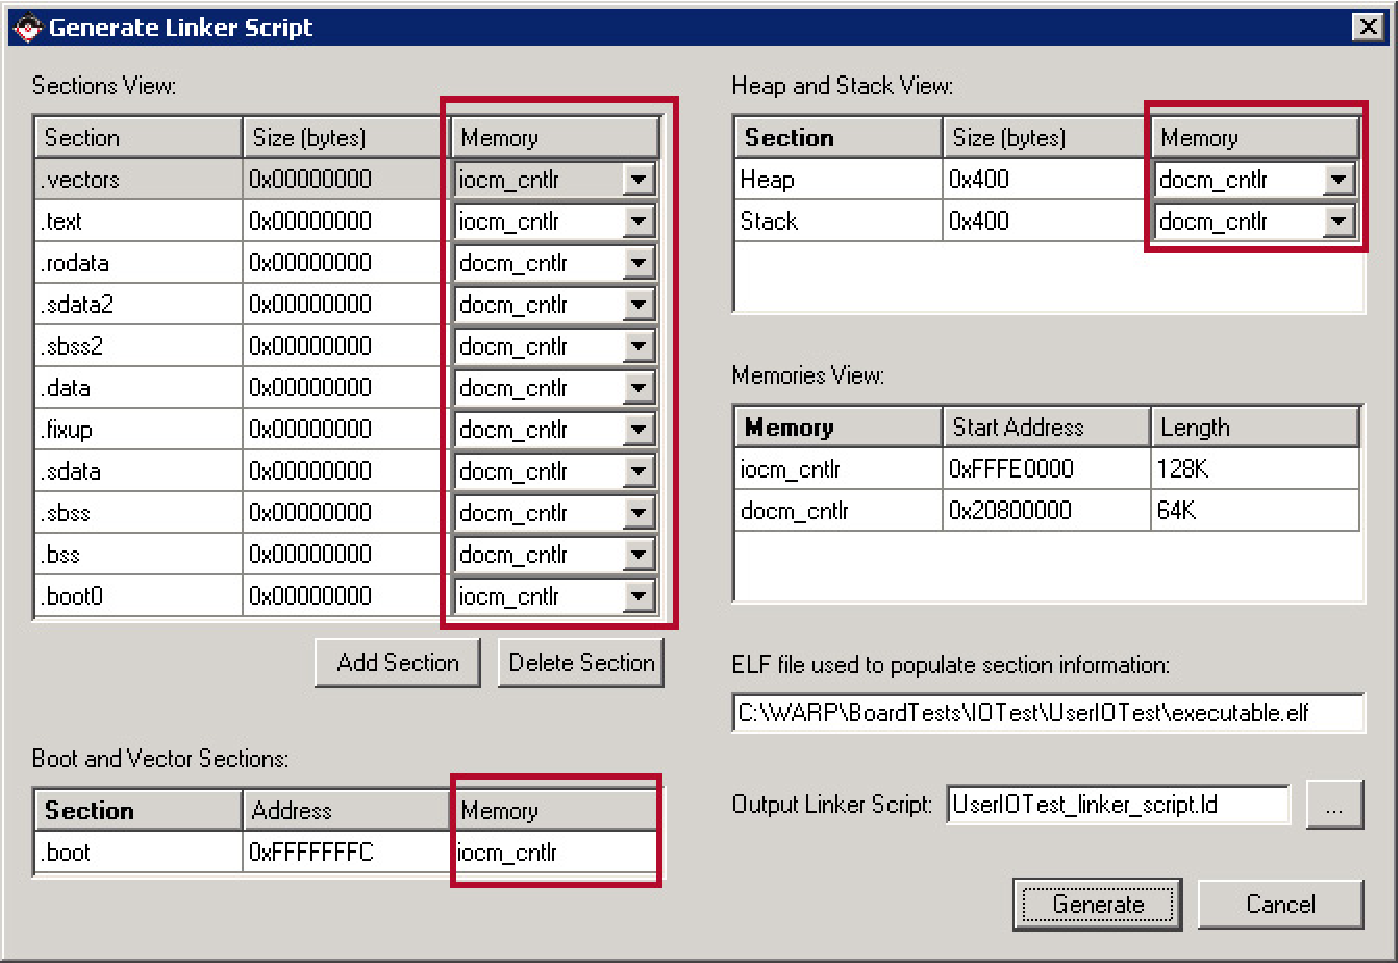
\includegraphics[width=.75\textwidth]{SWScreenshots/SW2p6b.pdf}
	\caption{Step 6 -- Set memory to iocm\_cntlr or docm\_cntlr}
	\label{fig:SW2p6b}
\end{figure}
			
			\newpage
			%Step 7%%%%%%%%%%%%%%%%%%%%%%%%%%%	
			\item Choose \textbf{Update Bitstream} by either accessing it through \textbf{Device Configuration} on the top menu, or by clicking on the toolbar button (it says ``Bram Init'' on it). This process will take 10-15 minutes depending on your computing speed. Longer may indicate an improper setup (esp. steps 4,5,6 of this section).
			
			
\begin{figure}[htbp]
	\centering
		\includegraphics[width=.70\textwidth]{SWScreenshots/SW2p7.pdf}
	\caption{Step 7 -- Update Bitstream}
	\label{fig:SW2p7}
\end{figure}

		
			%Step 8%%%%%%%%%%%%%%%%%%%%%%%%%%%	
			\item The file is now ready to download to the board.
		\end{enumerate}
For help, please refer to the Help/FAQ page.
